\chapter{Appendix B}
\thispagestyle{chapterBeginStyle}
\label{appendixB}

\section{Experimental results for Grover's algorithm}

Below we present experimental results of Grover's algorithm for \textit{n} qubits, where $n = 3$ and $n = 5$. Results were carried out using one borrowed qubit, which was necessary to implement $C^{n-1}Z$ gates. Tests were carried out on a classical computer simulating quantum computer, because architecture of real quantum computers did not allow to run larger quantum circuits. Although, for smaller circuits results received on a real quantum computer were analogous to these from a simulation.

On the horizontal axis of histograms are given binary representations of numbers received as results of experiments. The rightmost qubit is always equal to $|0\rangle$, because this is our borrowed qubit (it was not even measured at the end of the experiment). The rest is written as a typical binary number (the rightmost qubit is the least significant one). The height of each bar represents a percentage of receiving each number in all of the experiments. We denote by \textit{m} number of iterations of Grover's algorithm (how many times $U_f$ and $U_s$ operators were applied). Each quantum circuit, for given \textit{m}, was launched 1000 times.

We can see, that the algorithm gives the best results for number of iterations equal to $O(\sqrt{N}) = O(\sqrt{2^n})$. For $n = 3$ we obtained the best result for 6 iterations, and for $n = 5$ for 7 iterations. These are equal to about $2.12 \sqrt{N}$ and $1.24 \sqrt{N}$ accordingly. We can see, that factor standing next to the $\sqrt{N}$ has declined even for such small difference in number of qubits and we can assume, that it will continue to drop for increasing number of qubits. Moreover, we can see that when we apply more than $O(\sqrt{N})$ iterations, a decline in the percentage share of the item we were looking for appears.

\newpage
\begin{landscape}
\begin{table}[ht]
    \begin{tabular}{c c} 
        \hline
        n = 3, m = 1 & n = 3, m = 2 \\ \hline
        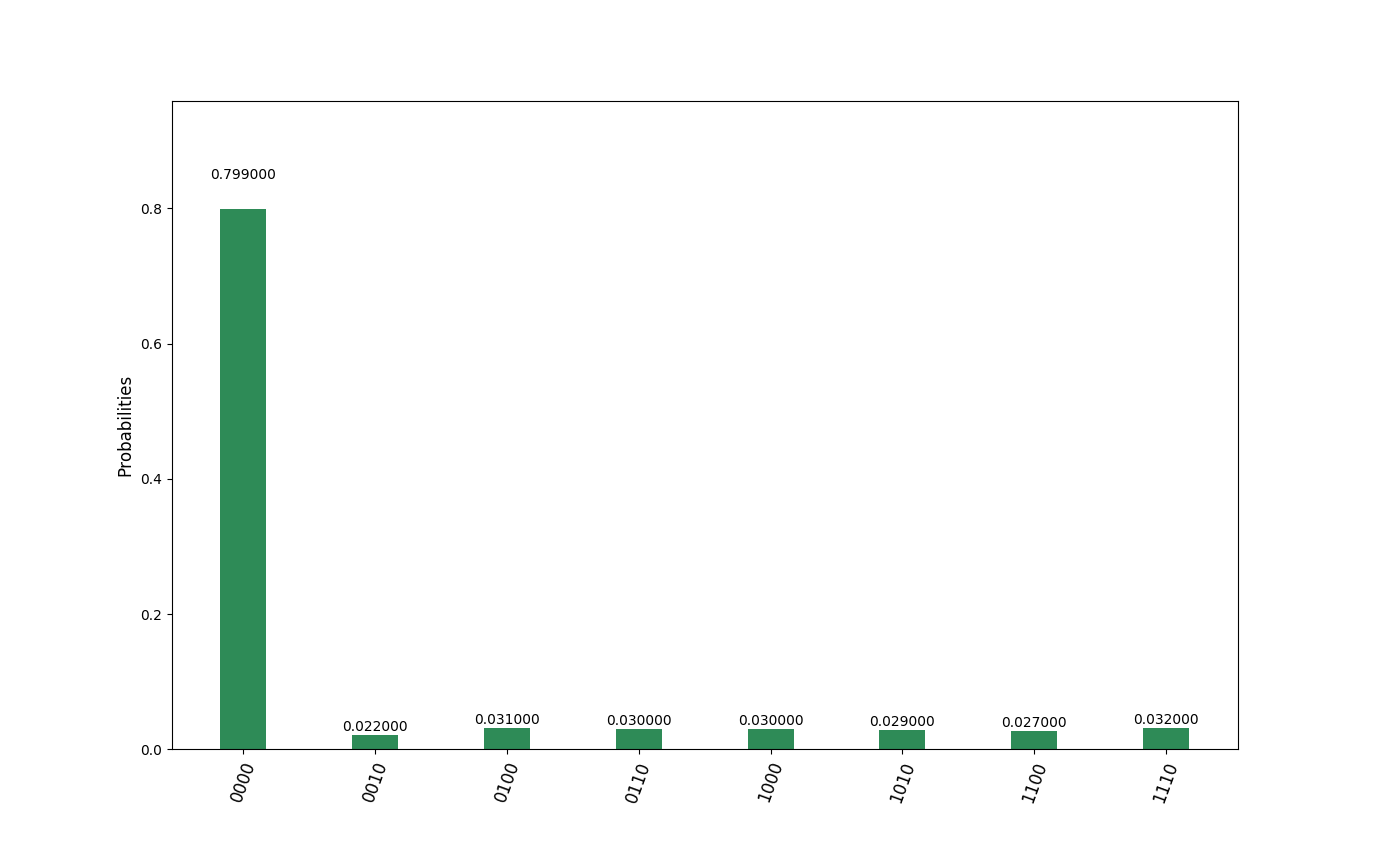
\includegraphics[scale=0.32]{Grover_results/Grover_n=3,m=1.png} & 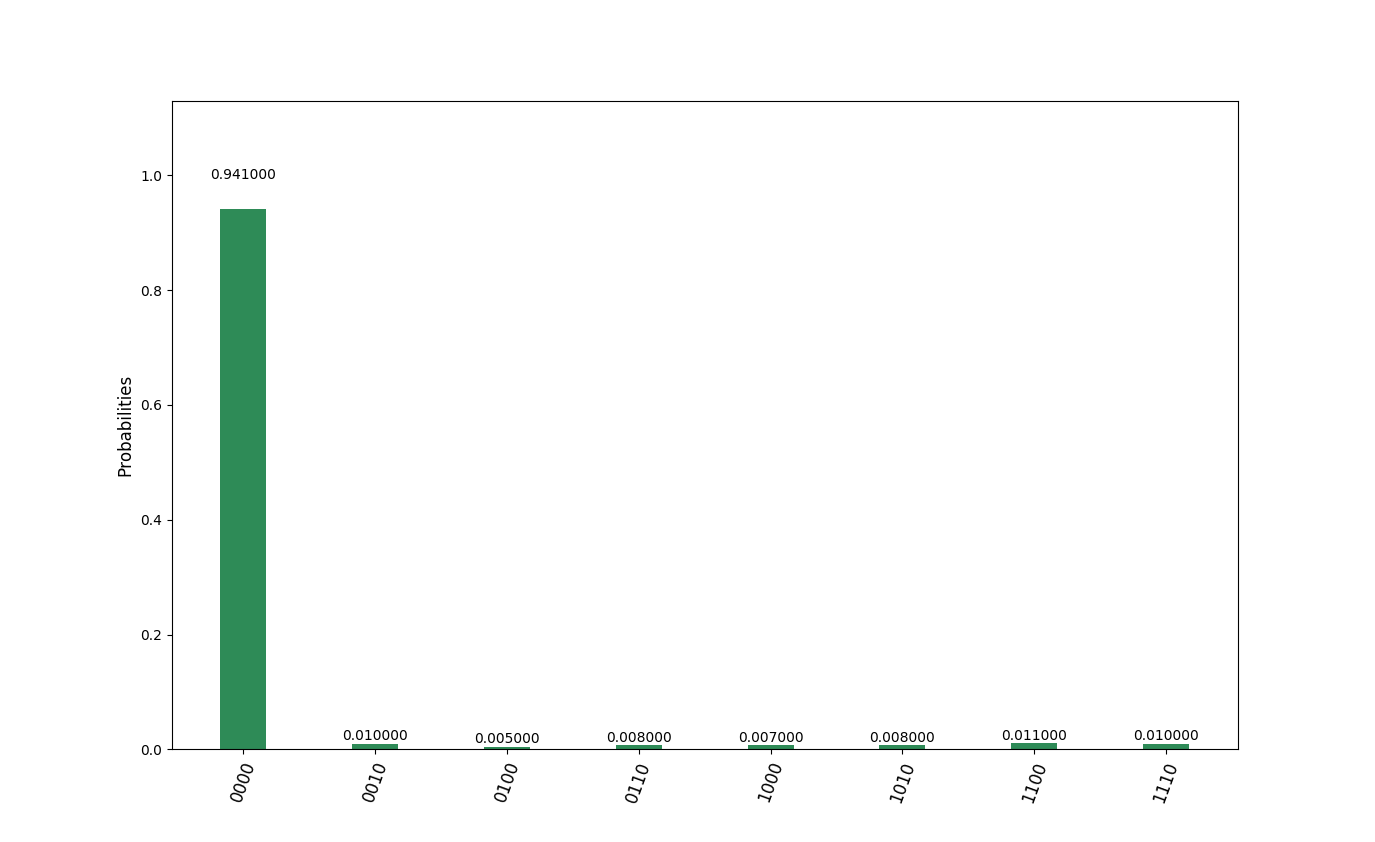
\includegraphics[scale=0.32]{Grover_results/Grover_n=3,m=2.png} \\ \hline
        n = 3, m = 3 & n = 3, m = 4 \\ \hline
        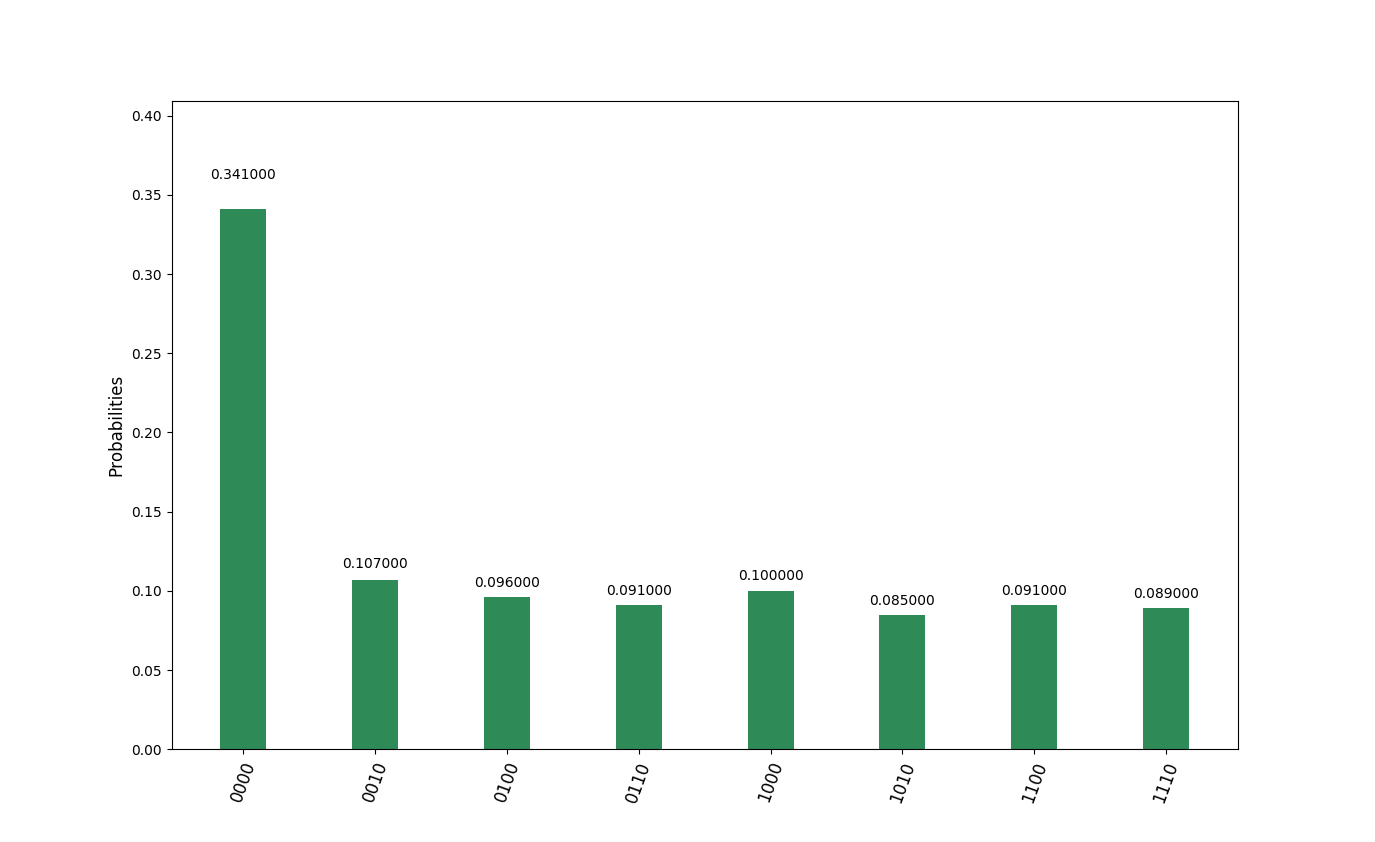
\includegraphics[scale=0.32]{Grover_results/Grover_n=3,m=3.png} & 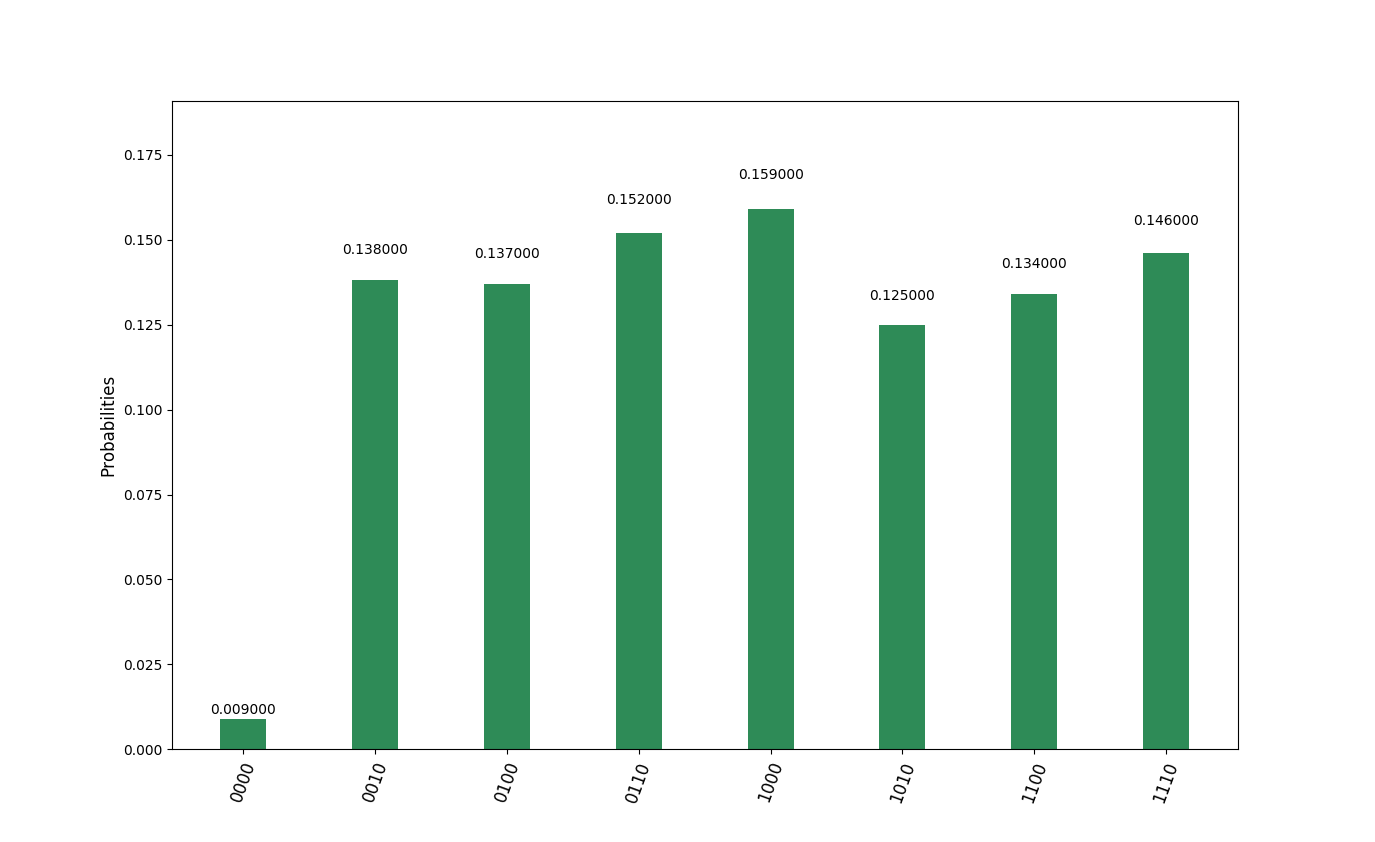
\includegraphics[scale=0.32]{Grover_results/Grover_n=3,m=4.png} \\ \hline
    \end{tabular}
\end{table}
\end{landscape}

\newpage
\begin{landscape}
\begin{table}[ht]
    \begin{tabular}{c c} 
        \hline
        n = 3, m = 5 & n = 3, m = 6 \\ \hline
        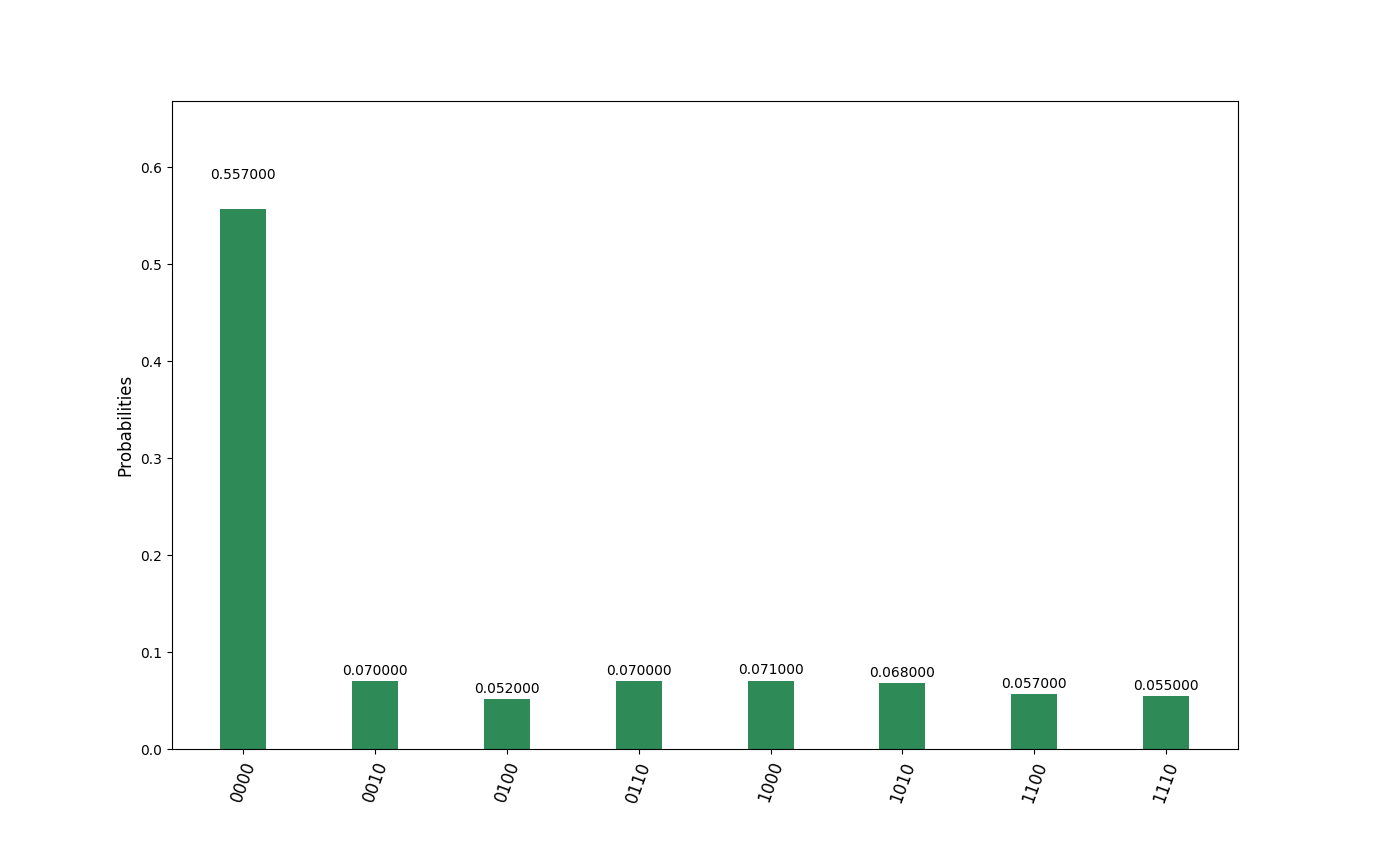
\includegraphics[scale=0.32]{Grover_results/Grover_n=3,m=5.png} & 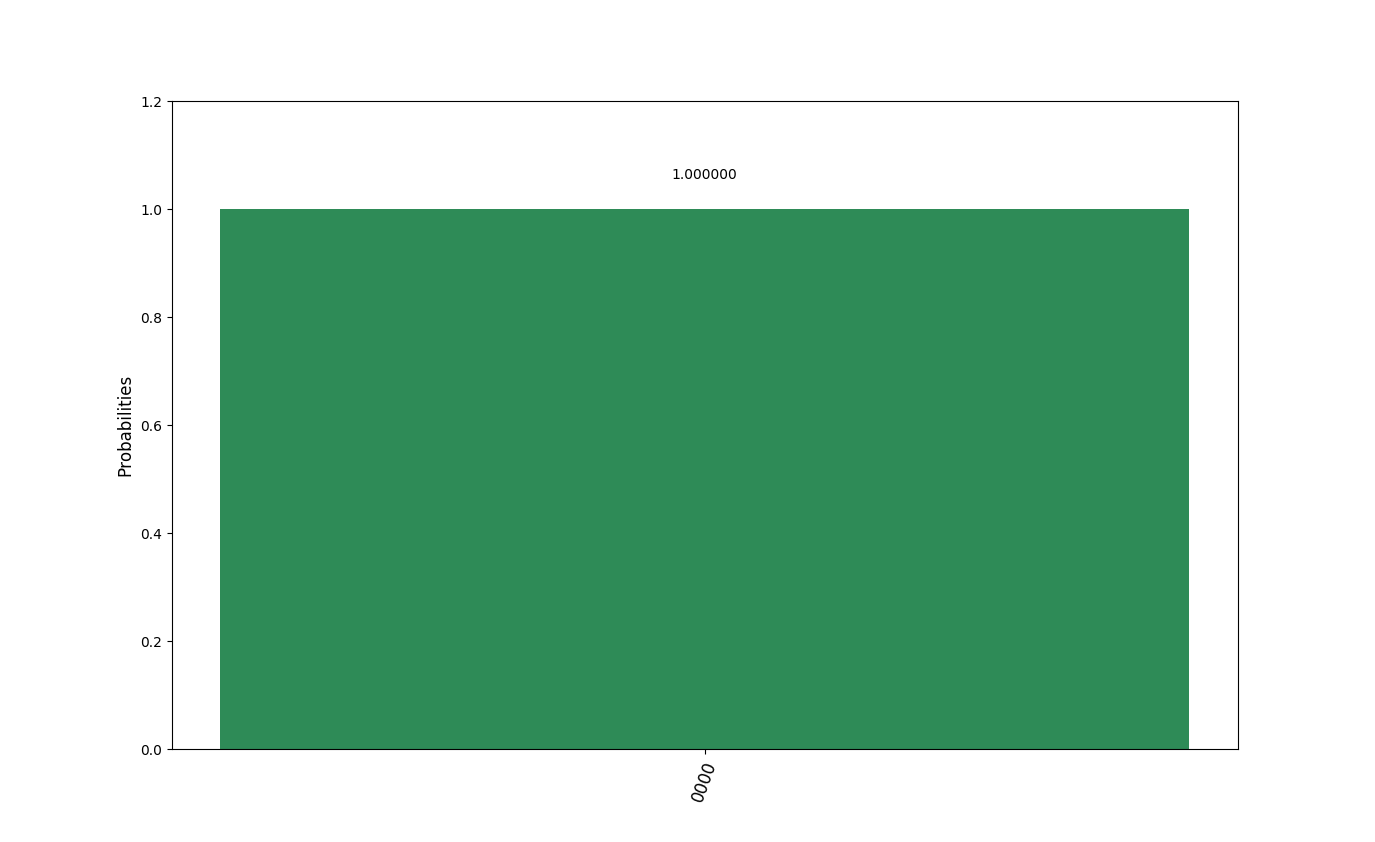
\includegraphics[scale=0.32]{Grover_results/Grover_n=3,m=6.png} \\ \hline
        n = 3, m = 7 & n = 3, m = 8 \\ \hline
        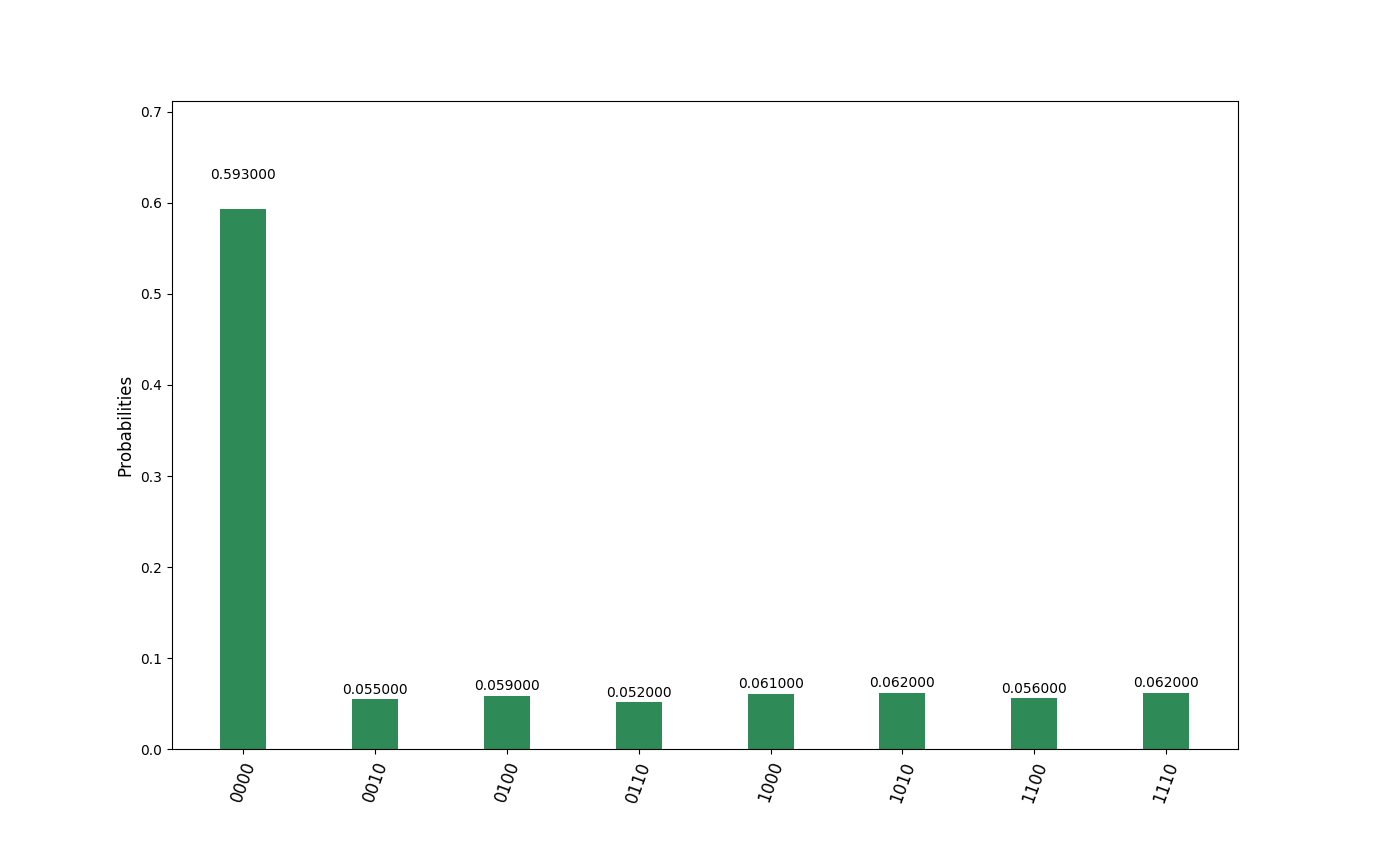
\includegraphics[scale=0.32]{Grover_results/Grover_n=3,m=7.png} & 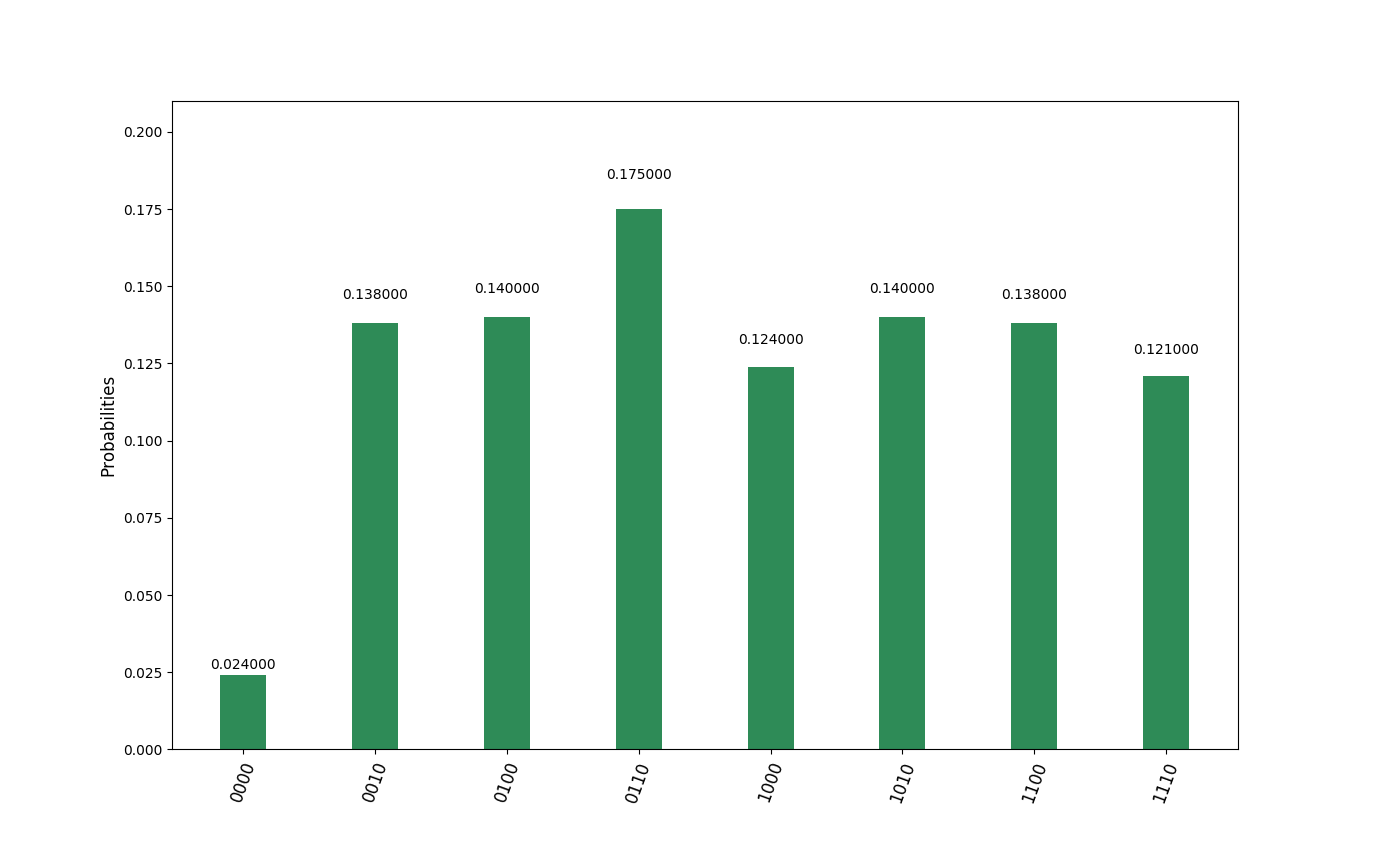
\includegraphics[scale=0.32]{Grover_results/Grover_n=3,m=8.png} \\ \hline
    \end{tabular}
\end{table}
\end{landscape}

\newpage
\begin{landscape}
\begin{table}[ht]
    \begin{tabular}{c c} 
        \hline
        n = 3, m = 9 & n = 3, m = 10 \\ \hline
        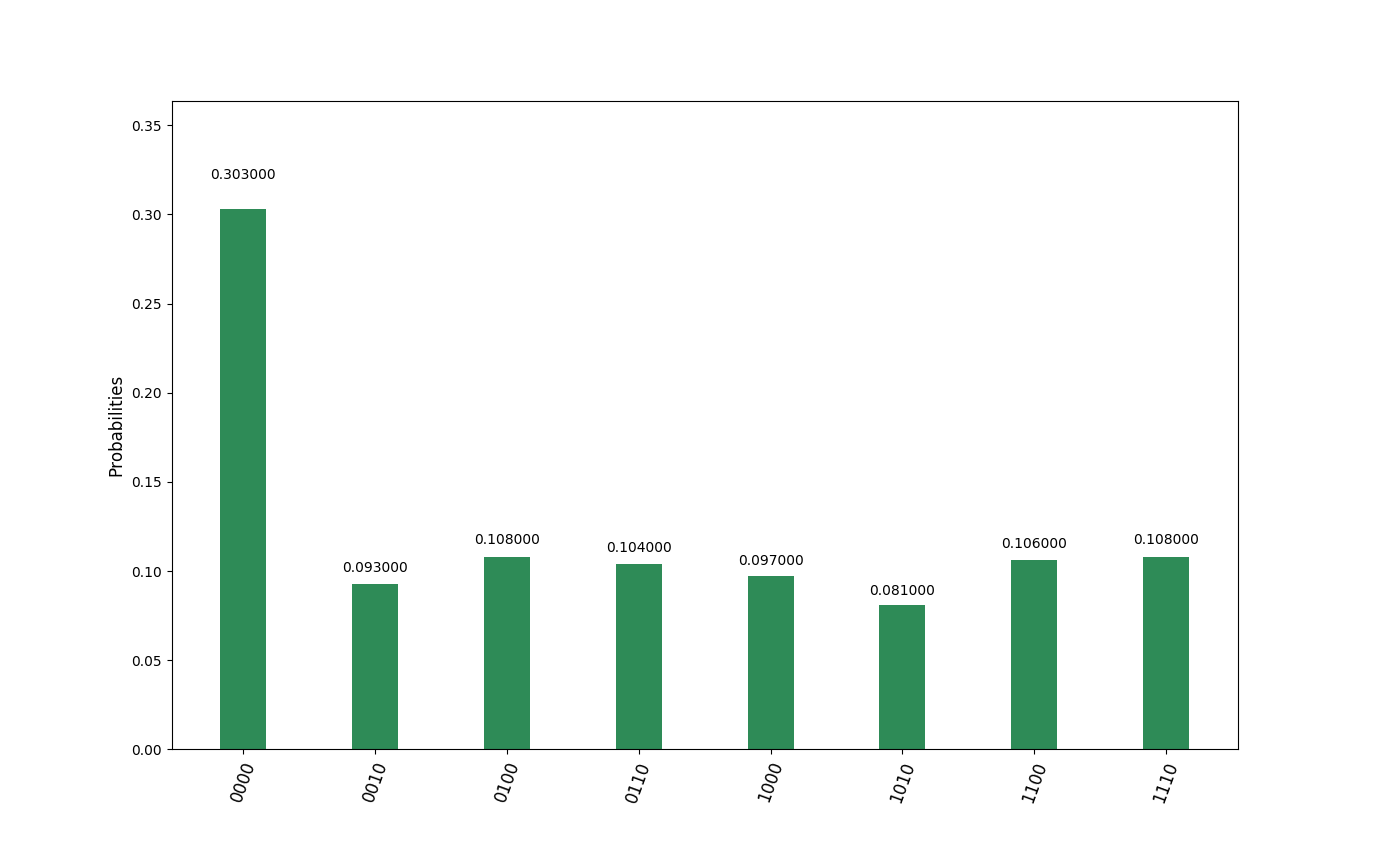
\includegraphics[scale=0.32]{Grover_results/Grover_n=3,m=9.png} & 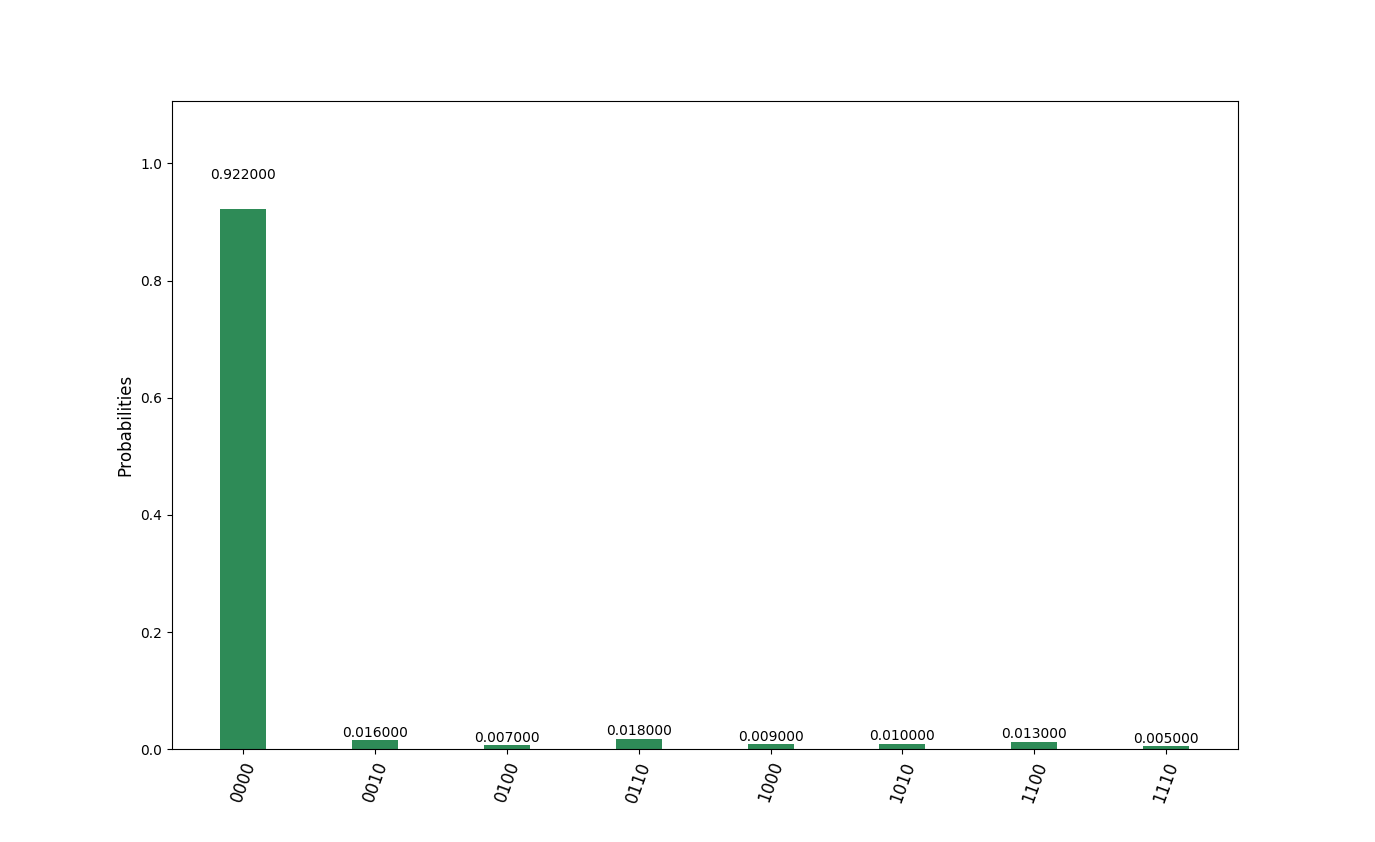
\includegraphics[scale=0.32]{Grover_results/Grover_n=3,m=10.png} \\ \hline
        n = 3, m = 11 & n = 3, m = 12 \\ \hline
        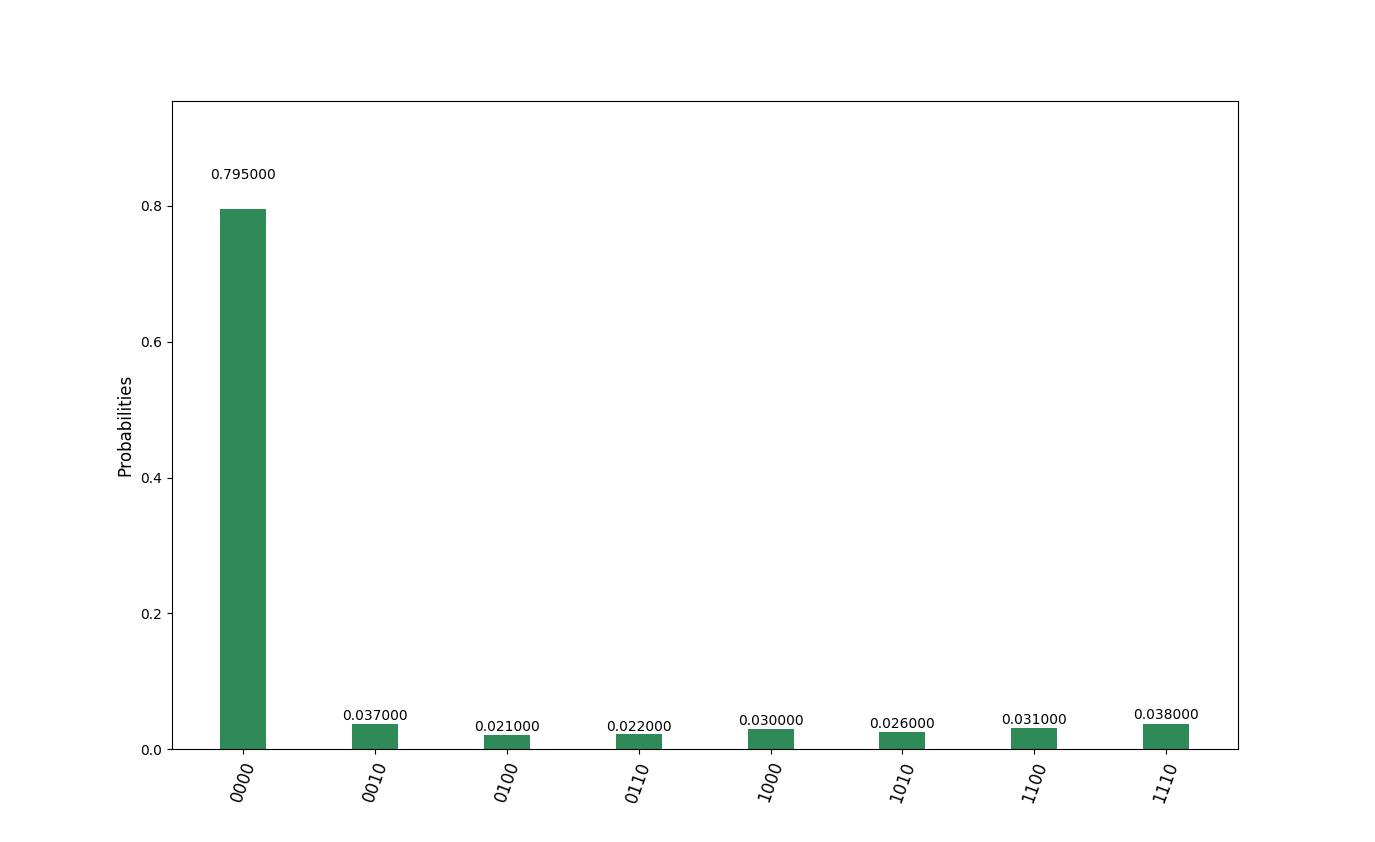
\includegraphics[scale=0.32]{Grover_results/Grover_n=3,m=11.png} & 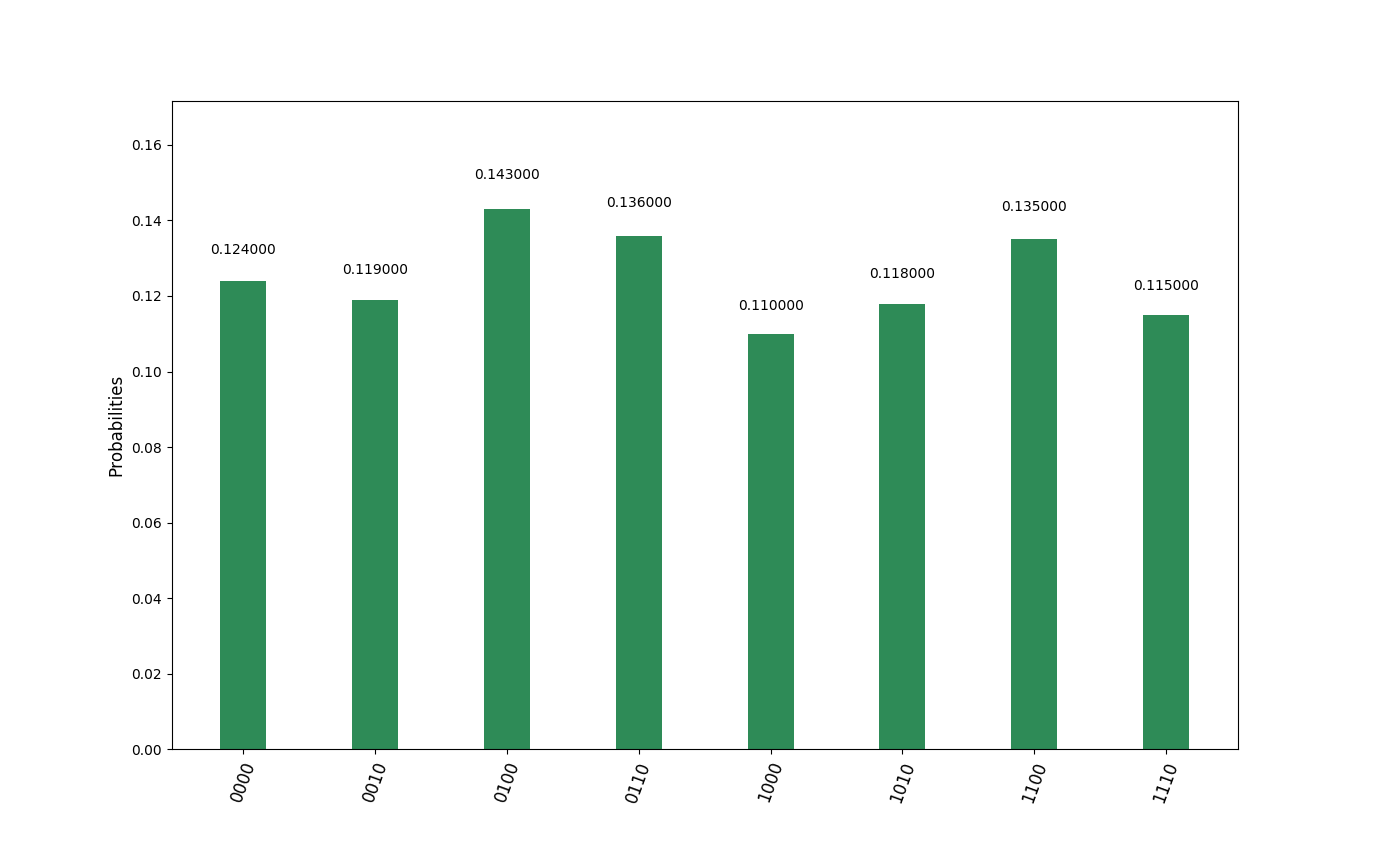
\includegraphics[scale=0.32]{Grover_results/Grover_n=3,m=12.png} \\ \hline
    \end{tabular}
\end{table}
\end{landscape}

\newpage
\begin{landscape}
\begin{table}[ht]
    \begin{tabular}{c c} 
        \hline
        n = 5, m = 1 & n = 5, m = 2 \\ \hline
        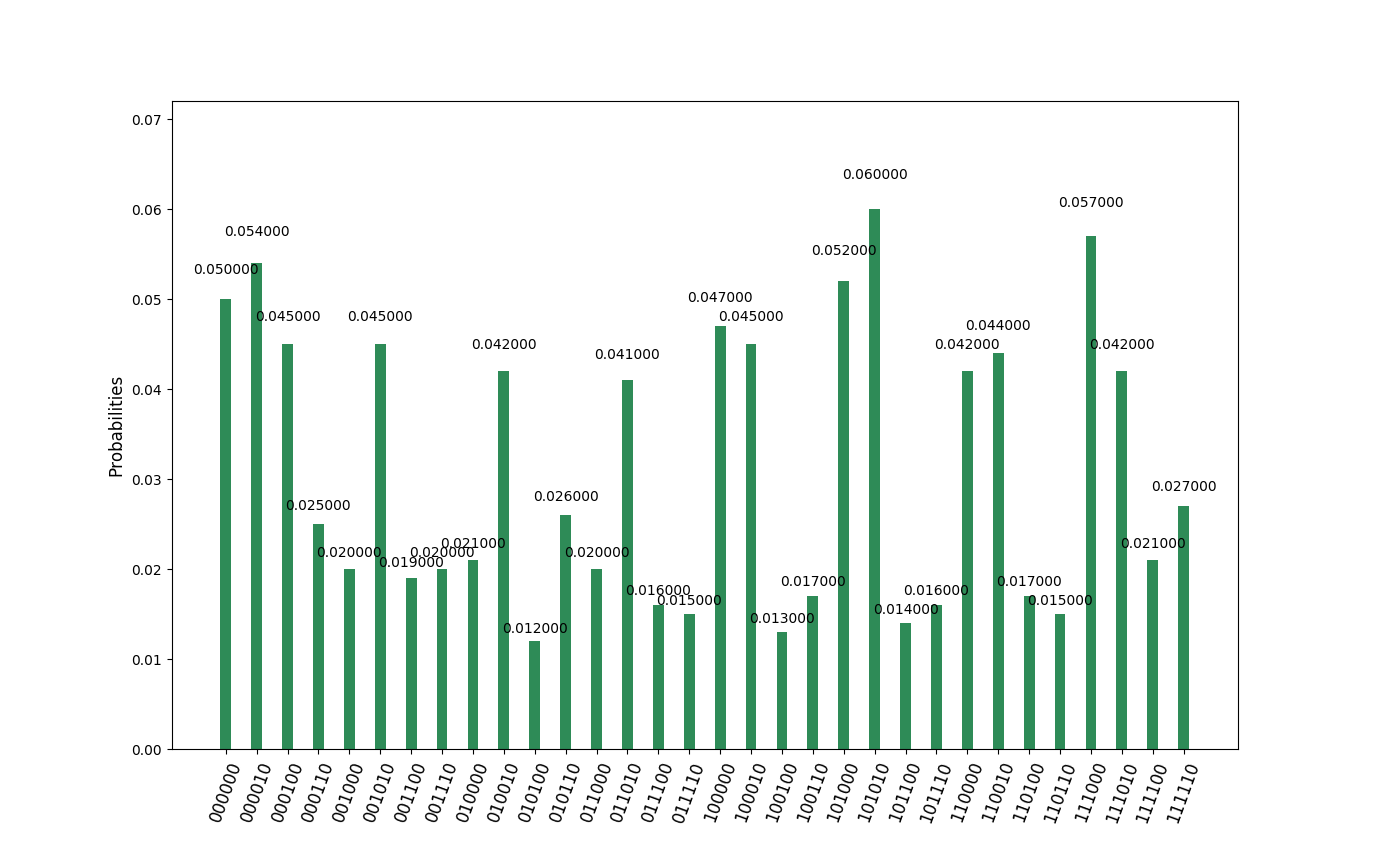
\includegraphics[scale=0.32]{Grover_results/Grover_n=5,m=1.png} & 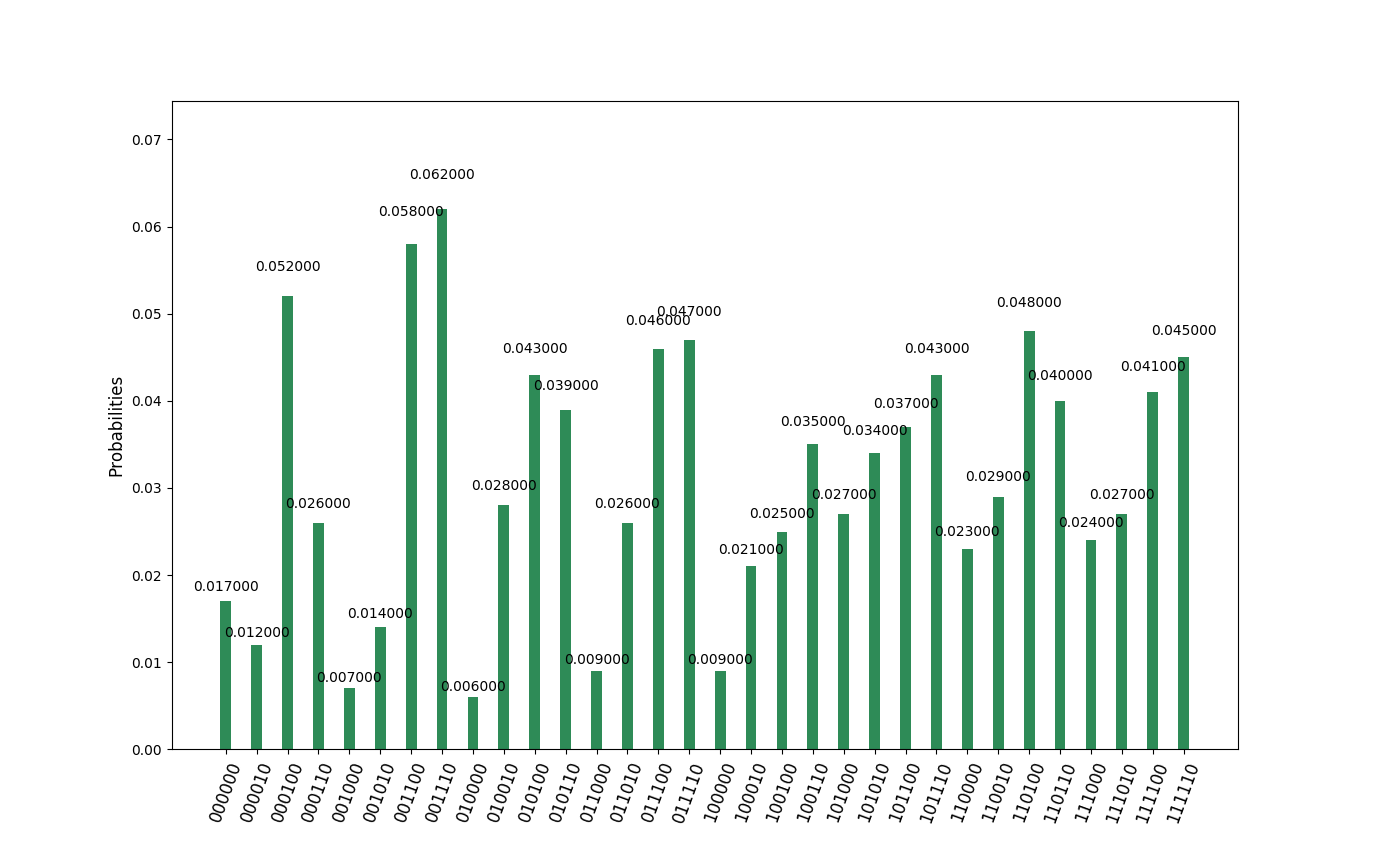
\includegraphics[scale=0.32]{Grover_results/Grover_n=5,m=2.png} \\ \hline
        n = 5, m = 3 & n = 5, m = 4 \\ \hline
        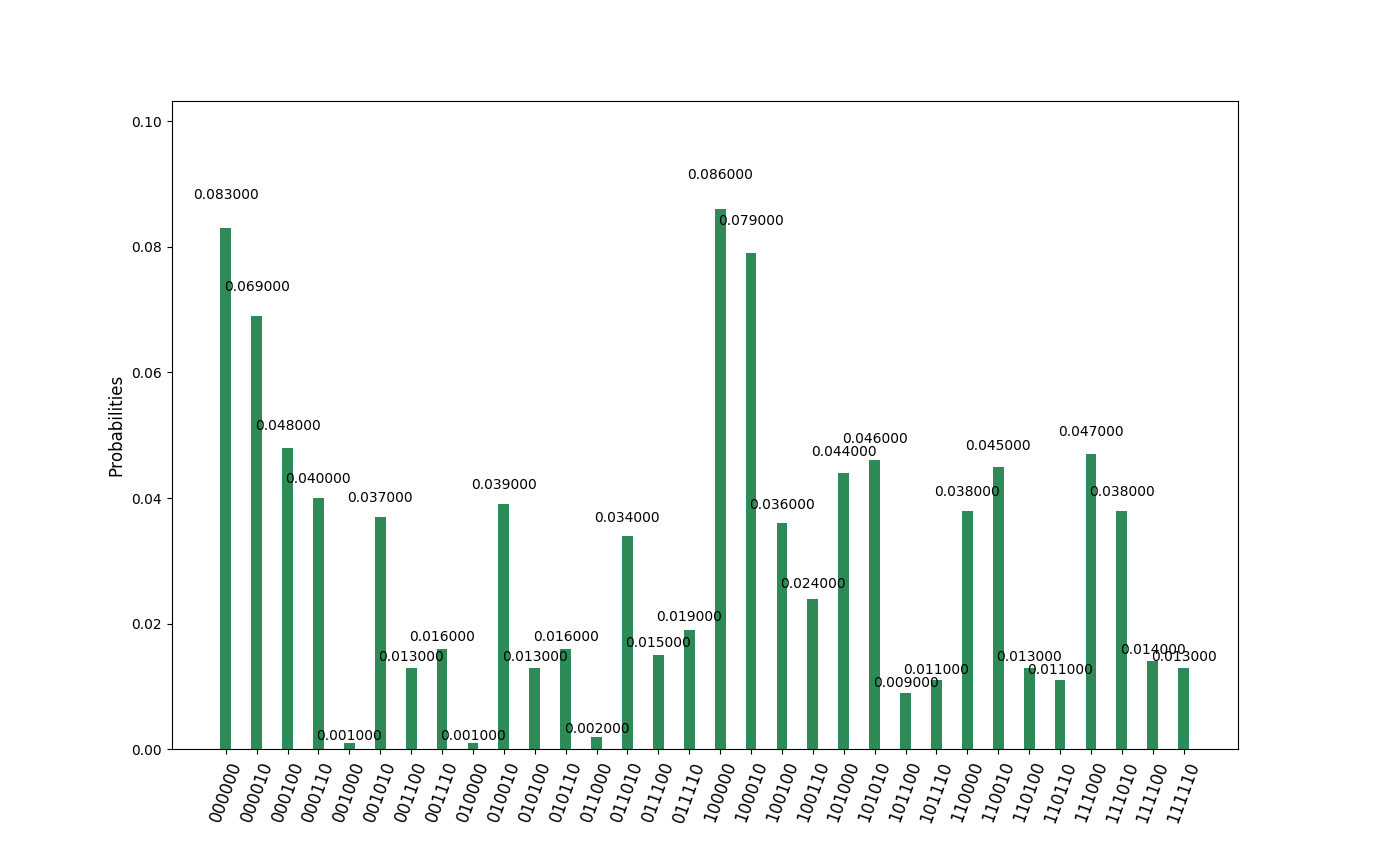
\includegraphics[scale=0.32]{Grover_results/Grover_n=5,m=3.png} & 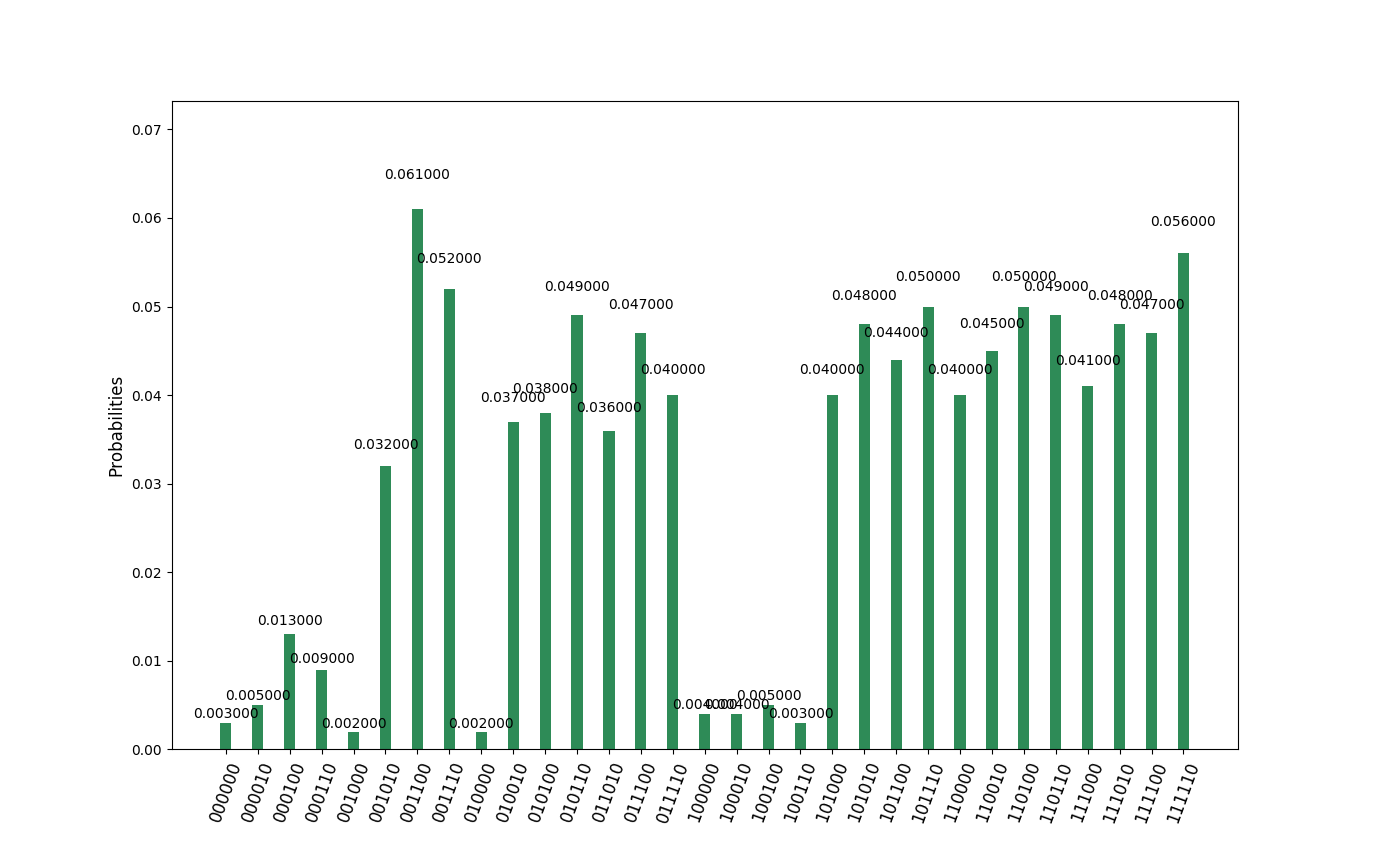
\includegraphics[scale=0.32]{Grover_results/Grover_n=5,m=4.png} \\ \hline
    \end{tabular}
\end{table}
\end{landscape}

\newpage
\begin{landscape}
\begin{table}[ht]
    \begin{tabular}{c c} 
        \hline
        n = 5, m = 5 & n = 5, m = 6 \\ \hline
        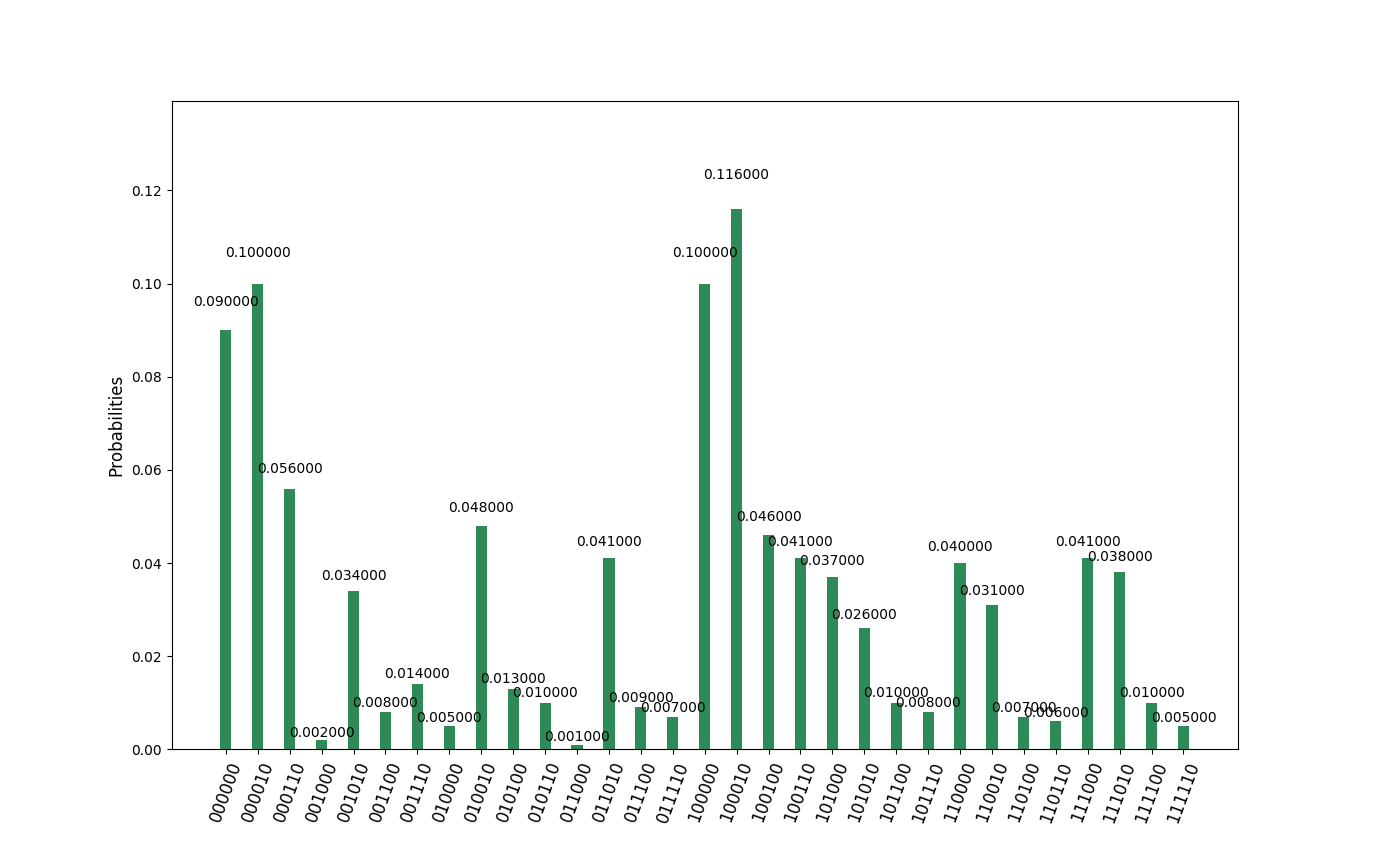
\includegraphics[scale=0.32]{Grover_results/Grover_n=5,m=5.png} & 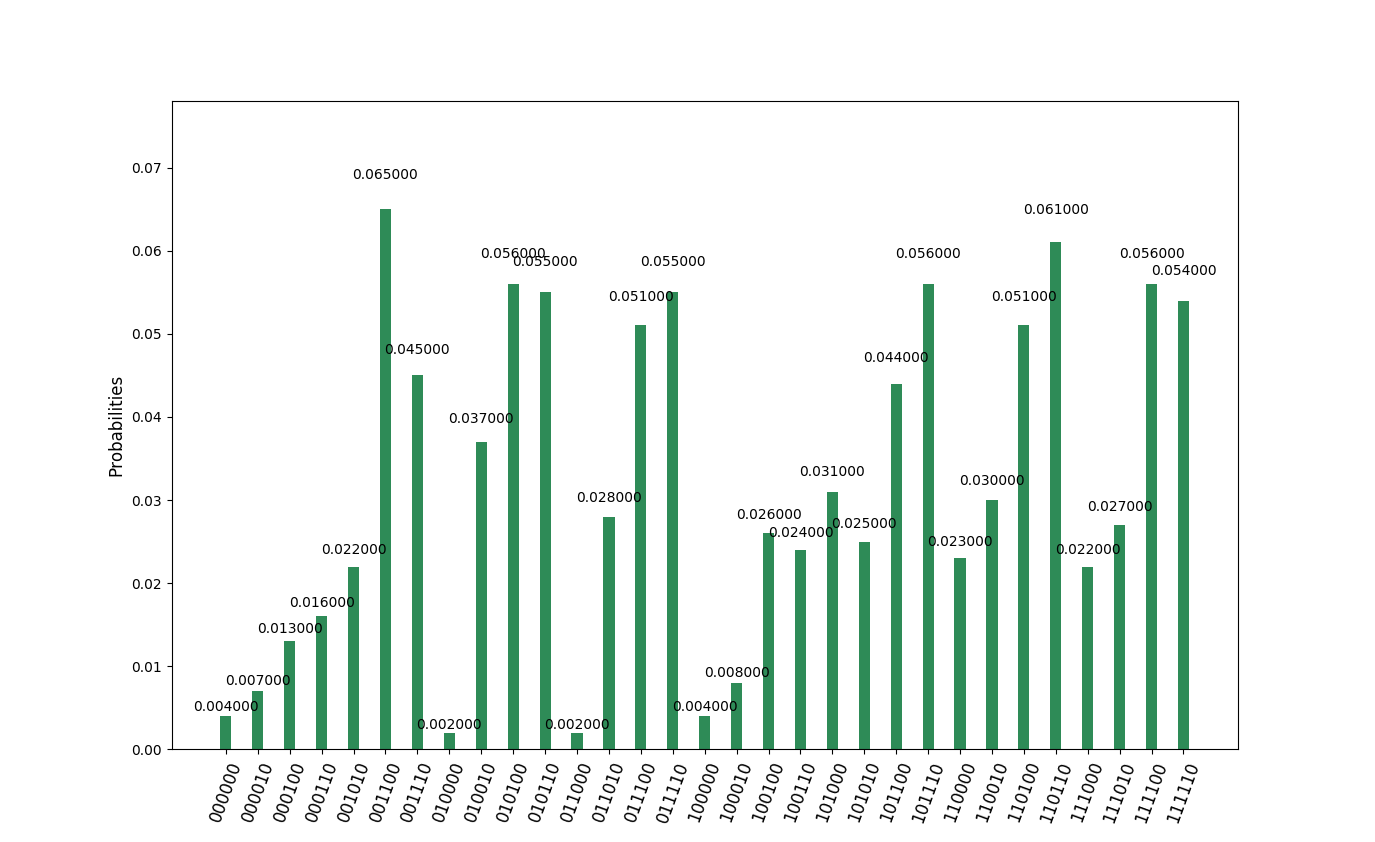
\includegraphics[scale=0.32]{Grover_results/Grover_n=5,m=6.png} \\ \hline
        n = 5, m = 7 & n = 5, m = 8 \\ \hline
        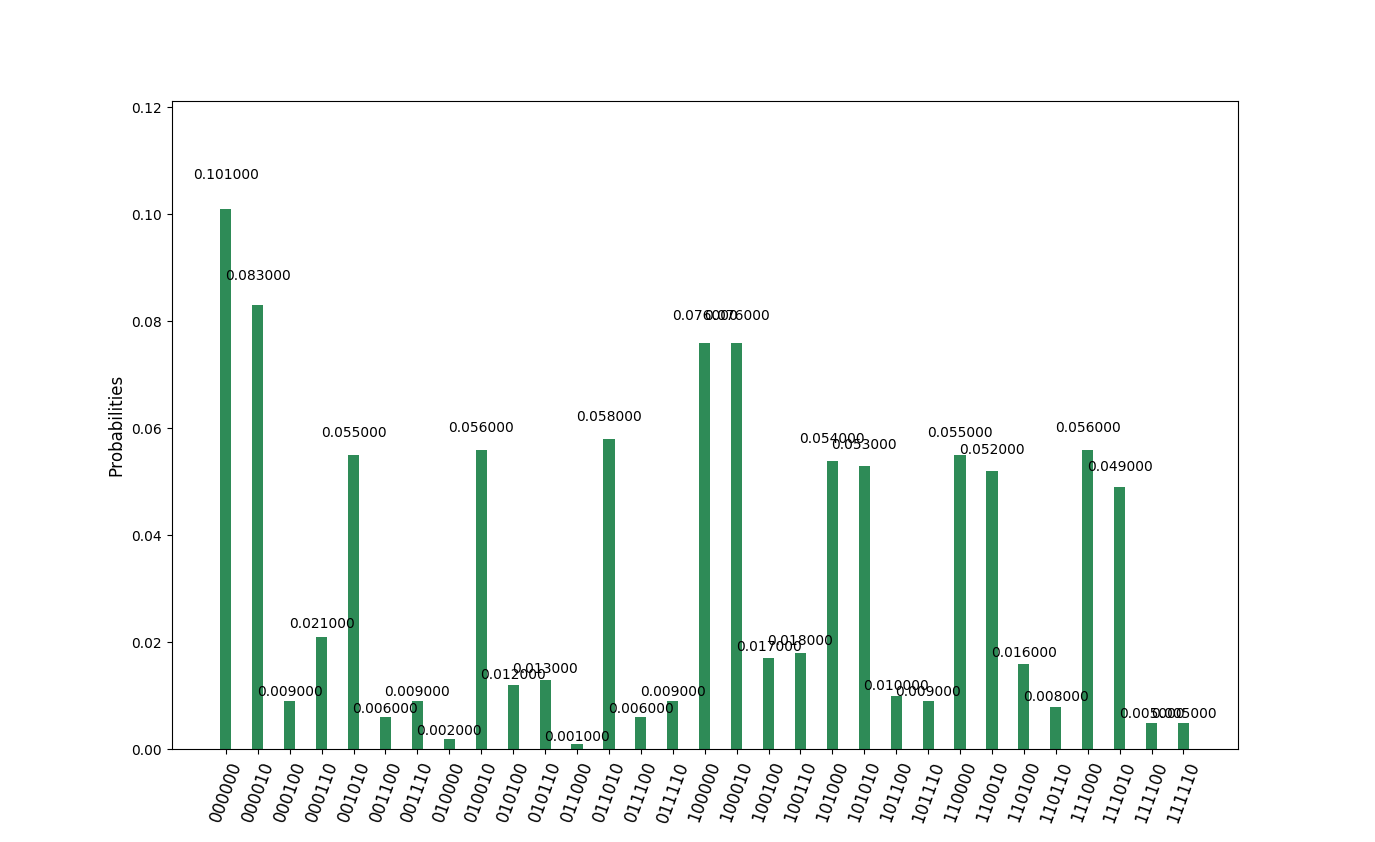
\includegraphics[scale=0.32]{Grover_results/Grover_n=5,m=7.png} & 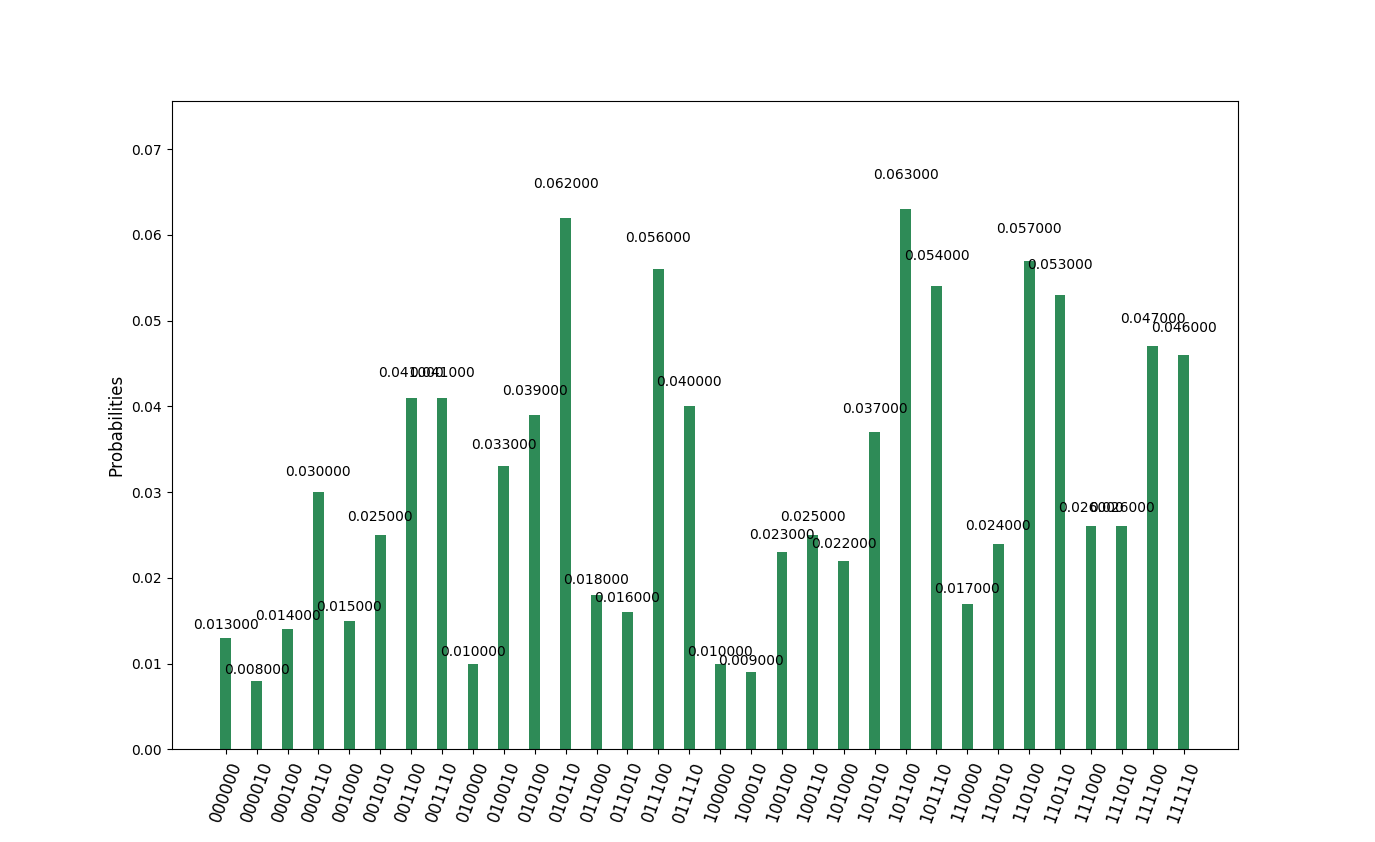
\includegraphics[scale=0.32]{Grover_results/Grover_n=5,m=8.png} \\ \hline
    \end{tabular}
\end{table}
\end{landscape}

\newpage
\begin{landscape}
\begin{table}[ht]
    \begin{tabular}{c c} 
        \hline
        n = 5, m = 9 & n = 5, m = 10 \\ \hline
        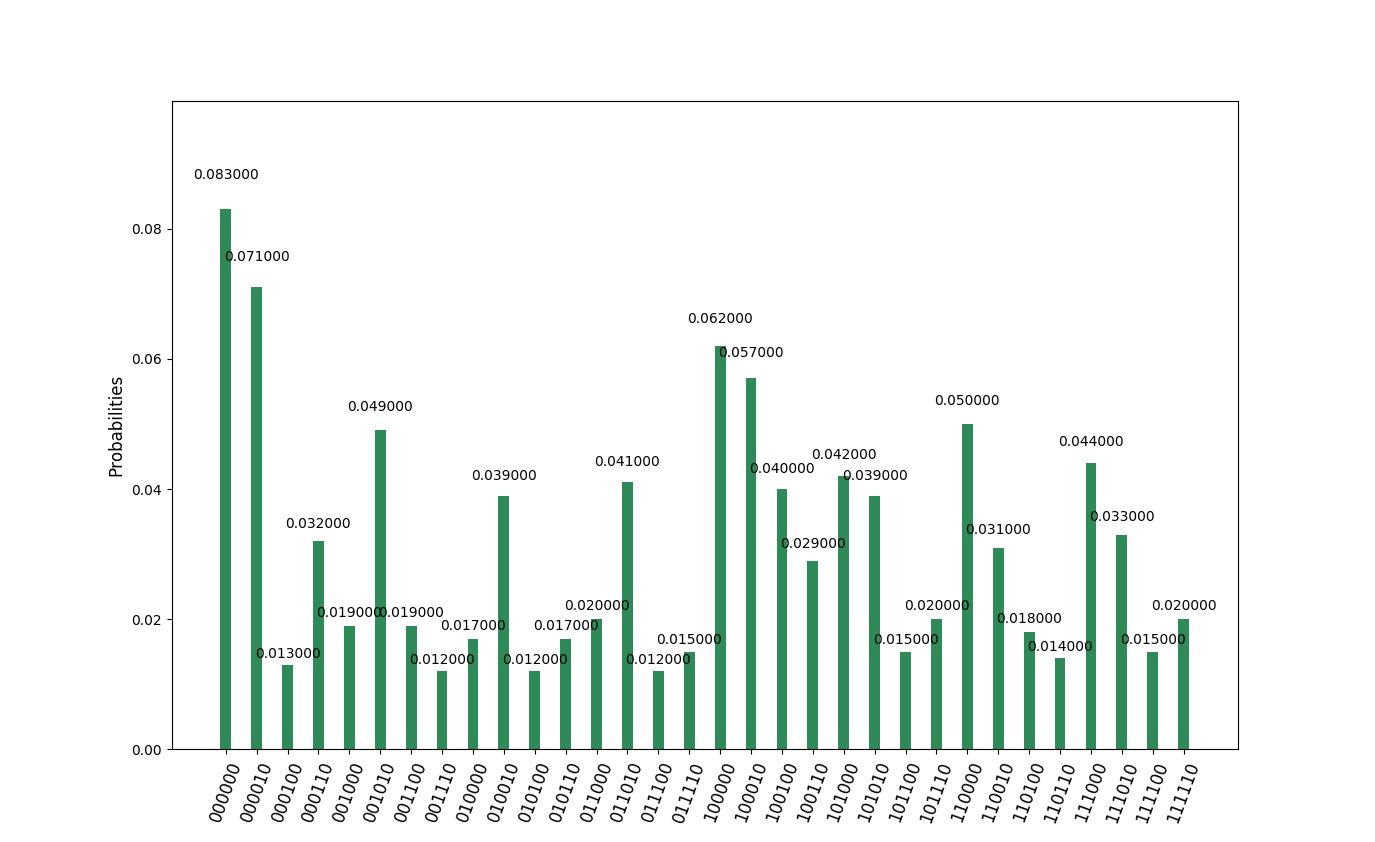
\includegraphics[scale=0.32]{Grover_results/Grover_n=5,m=9.png} & 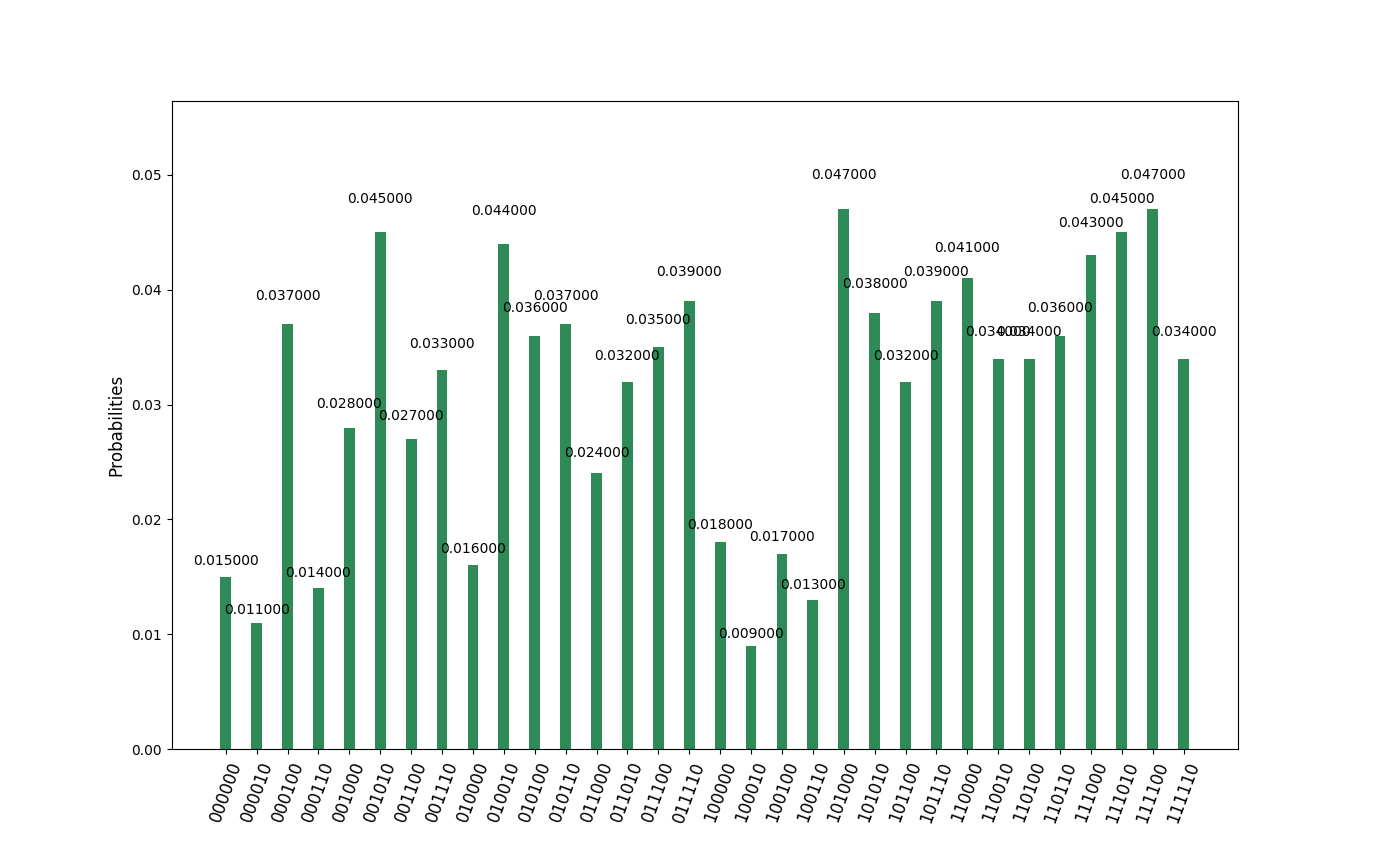
\includegraphics[scale=0.32]{Grover_results/Grover_n=5,m=10.png} \\ \hline
        n = 5, m = 11 & n = 5, m = 12 \\ \hline
        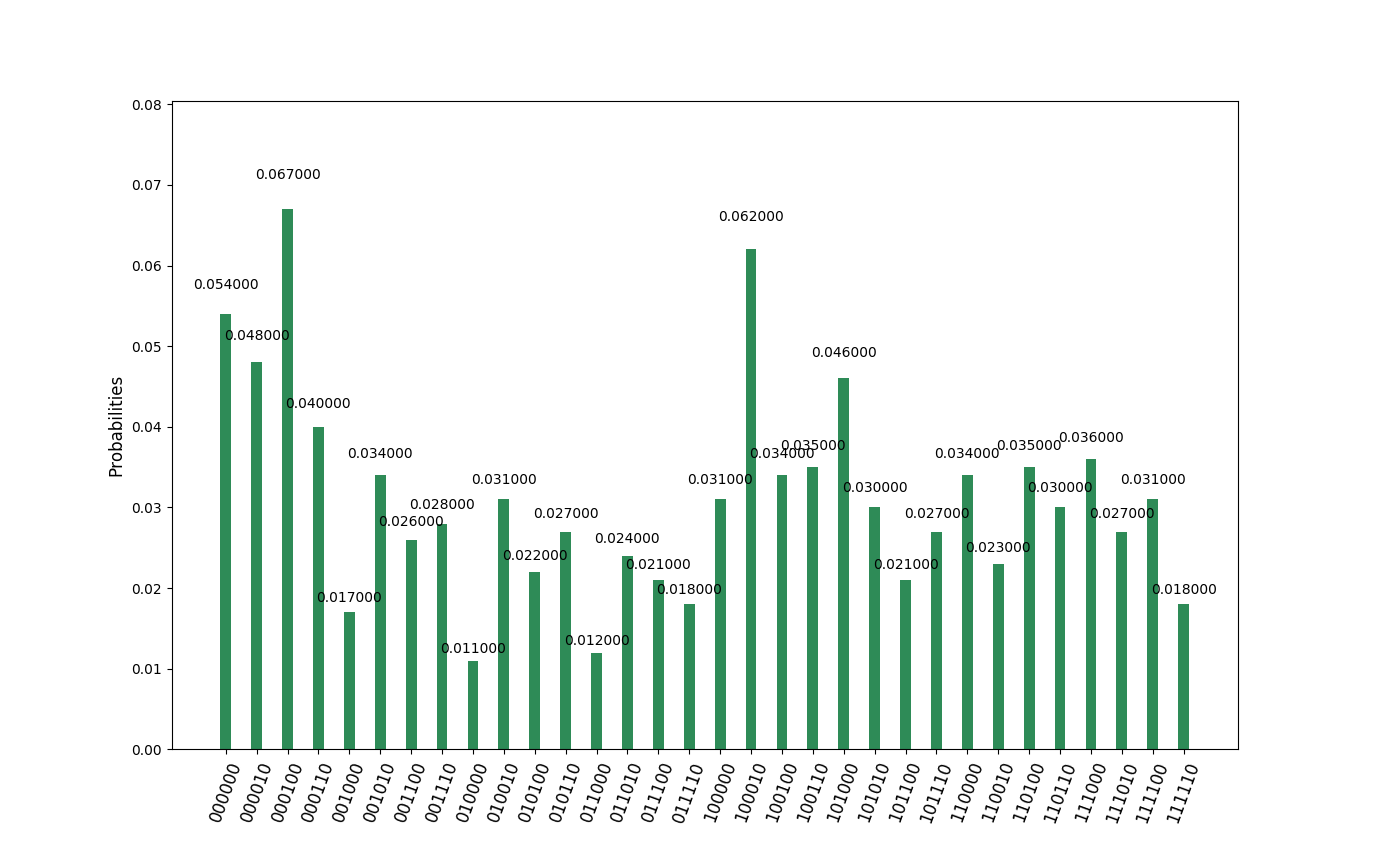
\includegraphics[scale=0.32]{Grover_results/Grover_n=5,m=11.png} & 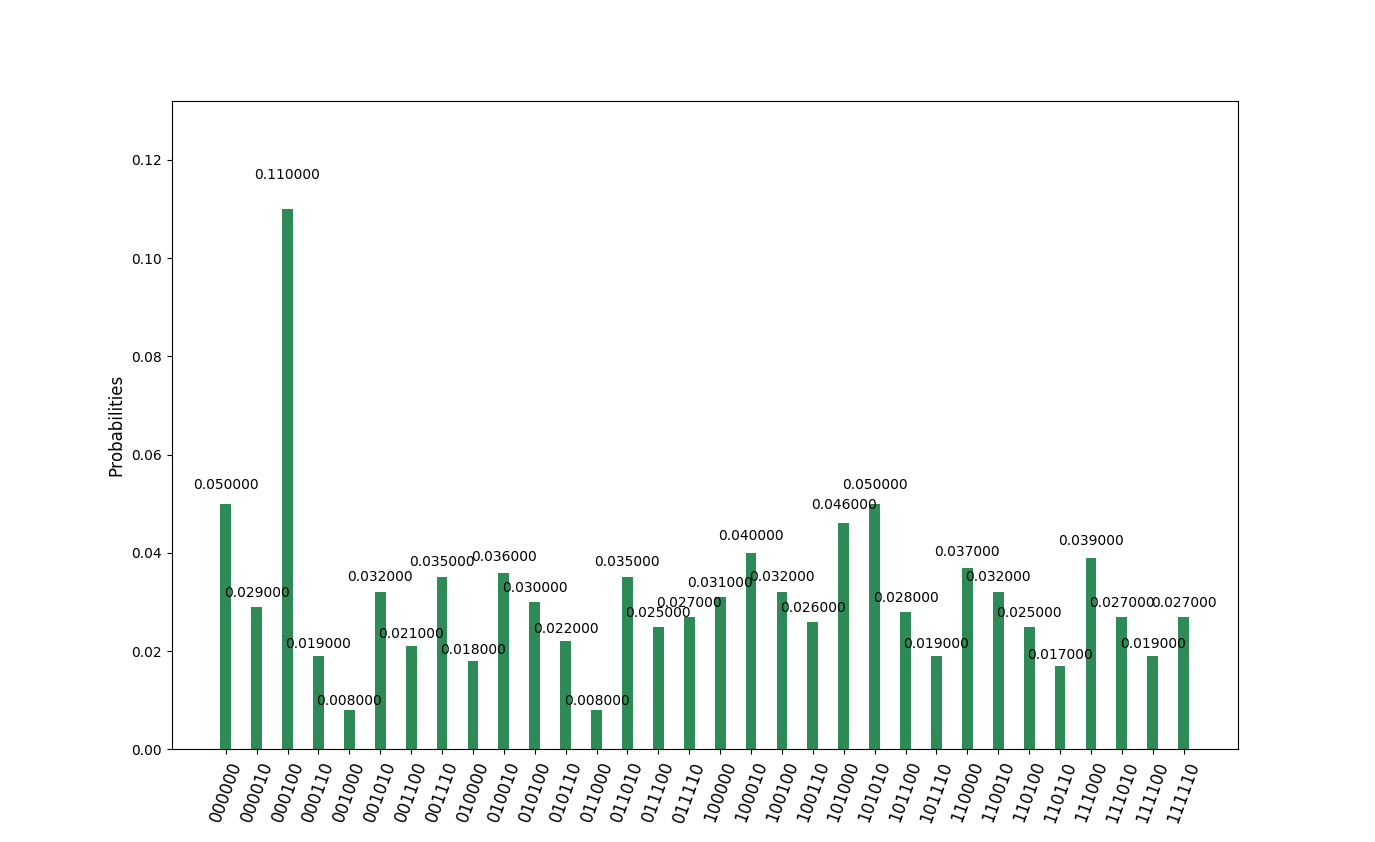
\includegraphics[scale=0.32]{Grover_results/Grover_n=5,m=12.png} \\ \hline
    \end{tabular}
\end{table}
\end{landscape}